%! Author = zlapik
%! Date = 01/04/2023
% Help
% \cmd[option]{arguments}

% Preamble
\documentclass[8pt, landscape]{article}
\pagestyle{empty}

% Packages
\usepackage{lmodern}
\usepackage[T1]{fontenc}
\usepackage{amsmath}
\usepackage{amsfonts}
\usepackage{amssymb}
\usepackage{amsthm}
\usepackage{graphicx}
\usepackage{hyperref}
\usepackage{cleveref}
\hypersetup{
    colorlinks=true,
    linkcolor=blue,
    filecolor=magenta,
    urlcolor=red,
    citecolor=green,
    pdftitle={Reinforcement Learning Cheatsheet},
}
\usepackage{listings}
\usepackage{mathtools}
\usepackage{multirow}
\usepackage{paralist}
\usepackage[landscape]{geometry}
\usepackage{lipsum}
\usepackage{tikz}
\usepackage{multicol}
\usepackage{pgfplots}
\usepackage{calc}
\usepackage{algorithm2e}
\usepackage{float}
\usepackage[utf8]{inputenc}
\usetikzlibrary{arrows.meta,shadows,positioning}

% Definitions
\newcommand{\lengthfromedge}{0.5cm}
\newcommand{\textfontsize}{8pt}
\makeatletter
\renewcommand{\section}{\@startsection{section}{1}{0mm}%
{-1ex plus -.5ex minus -.2ex}%
{0.5ex plus .2ex}%x
{\normalfont\large\bfseries}}
\renewcommand{\subsection}{\@startsection{subsection}{2}{0mm}%
{-1explus -.5ex minus -.2ex}%
{0.5ex plus .2ex}%
{\normalfont\normalsize\bfseries}}
\renewcommand{\subsubsection}{\@startsection{subsubsection}{3}{0mm}%
{-1ex plus -.5ex minus -.2ex}%
{1ex plus .2ex}%
{\normalfont\small\bfseries}}
\newcommand\numberthis{\addtocounter{equation}{1}\tag{\theequation}}
\makeatother
\DeclareMathOperator*{\argmax}{argmax}

% Don't print section numbers
%\setcounter{secnumdepth}{0}

% Page setup
\geometry{top=\lengthfromedge,left=\lengthfromedge,right=\lengthfromedge,bottom=\lengthfromedge}

% Lists
\setlength{\parindent}{0pt}
\setlength{\parskip}{0pt plus 0.5ex}

% Tikz
\tikzset{
    frame/.style={
        rectangle, draw,
%        text width=6em,
        text centered,
        minimum height=3em,drop shadow,fill=white,
        rounded corners,
    },
    line/.style={
        draw, -{Latex},rounded corners=3mm,
    },
    fontscale/.style = {
        font=\relsize{#1}
    },
    block/.style = {
        rectangle,
        draw,
        text width=8em,
        text centered,
        rounded corners,
        minimum height=2.5em
    },
}

% Document
\begin{document}
    \raggedright
    \fontsize{\textfontsize}{\textfontsize}\selectfont

    \begin{multicols}{3}
        % Multicols Setup
        \setlength{\premulticols}{1pt}
        \setlength{\postmulticols}{0.1pt}
        \setlength{\multicolsep}{1pt}
        \setlength{\columnsep}{1pt}

        % Title
        \begin{center}
            \Large{Reinforcement Learning Cheat Sheet} \\
        \end{center}

        \section*{Summary of Notation}


        \section{Introduction}

        \subsection{Recap}
        foo:
        \begin{equation}
            \mathbb{E}[X] = \sum_{x_i} x_i \cdot Pr\{ X = x_i \}
        \end{equation}
        foo:
        \begin{equation}
            \mathbb{E}[X | Y = y_j] = \sum_{x_i} x_i \cdot Pr\{ X = x_i | Y = y_j\}
        \end{equation}
        foo:
        \begin{equation}
            \mathbb{E}[X | Y = y_j] = \sum_{z_k} Pr\{Z=z_k | Y = y_j\} \cdot \mathbb{E}[X|Y = y_j, Z = z_k]
        \end{equation}
%        $\mathbb{E}[X] \stackrel{.}{=} \sum_{x_i} x_i \cdot Pr\{ X = x_i \}$
%        $\mathbb{E}[X | Y = y_j] = \sum_{x_i} x_i \cdot Pr\{ X = x_i | Y = y_j\}$
%        $\mathbb{E}[X | Y = y_j] = \sum_{z_k} Pr\{Z=z_k | Y = y_j\} \cdot \mathbb{E}[X|Y = y_j, Z = z_k]$


        \section{Multi-armed Bandits}


        \section{Finite Markov Decision Process}

        \subsection{Agent-Environment Interaction}
        \begin{center}
            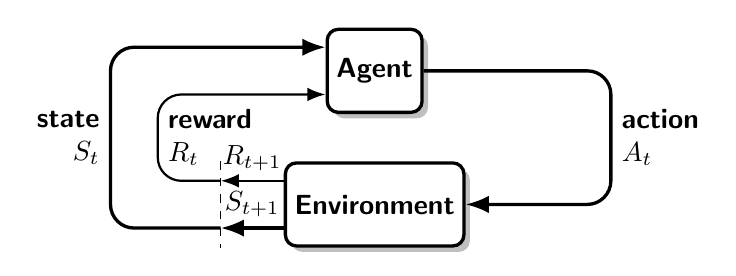
\begin{tikzpicture}[font=\sffamily\bfseries,very thick,node distance = 4cm]
                \node [frame] (agent) {Agent};
                \node [frame, below=0.6cm of agent] (environment) {Environment};
                \draw[line] (agent) -- ++ (3,0) |- (environment)
                node[right,pos=0.25,align=left] {action\\ $A_t$};
                \coordinate[left=8mm of environment] (P);
                \coordinate[above=3mm of environment.west] (ENW);
                \coordinate[below=3mm of environment.west] (ESW);
                \coordinate[above=3mm of agent.west] (ANW);
                \coordinate[below=3mm of agent.west] (ASW);
                \draw[thin,dashed] (P|-environment.north) -- (P|-environment.south);
                \draw[line] (ESW) -- (P |- ESW)
                node[midway,above]{$S_{t+1}$};
                \draw[line,thick] (ENW) -- (P |- ENW)
                node[midway,above]{$R_{t+1}$};
                \draw[line] (P |- ESW) -- ++ (-1.4,0) |- (ANW)
                node[left, pos=0.25, align=right] {state\\ $S_t$};
                \draw[line,thick] (P |- ENW) -- ++ (-0.8,0) |- (ASW)
                node[right,pos=0.25,align=left] {reward\\ $R_t$};
            \end{tikzpicture}
        \end{center}


        \section{Dynamic Programming}


        \section{Monte Carlo Methods}


        \section{Temporal-Difference Learning}


        \section{n-step Bootstrapping}


        \section{Planning and Learning}


        \section{On Policy Prediction with Approximation}


        \section{On Policy Control with Approximation}


        \section{Off Policy Prediction with Approximation}


        \section{Eligibility Traces}


        \section{Policy Gradient Methods}


        \section{Psychology}


        \section{Neuroscience}


        \section{Application and case studies}


        \section{Frontiers}
    \end{multicols}
\end{document}